

We return to the application of association screenings for categorical variables, and put the results in the previous section to use.

In particular, we focus on the exact-approximate support recovery problem (Theorem \ref{thm:chi-squared-exact-approx-boundary}), and demonstrate the consequences of its phase transition in GWAS.
We also derive efficient study designs that attain the necessary statistical signal sizes in the special (but fairly common) case of association tests on 2-by-2 contingency tables.

In order to do so, we must first connect the concept of ``statistical signal size'' $\lambda$ with some key quantities in association tests.
While the former is likely foreign to most practitioners, it is intimately linked with the concept of ``effect sizes'' --- or odds ratios --- in association studies, which are usually explicitly estimated and reported in the GWAS literature.
% We begin by characterizing the relationship between the two.

\subsection{Odds ratios and statistical power}
\label{subsec:odds-and-power}

% Unlike in additive models where the parameter $\mu$ has the interpretation of signal-to-noise ratios, the meaning of the signal sizes $\lambda$ in chi-square model is perhaps not as transparent.

Consider a 2-by-2 multinomial distribution with marginal probabilities of phenotypes $(\phi_1, \phi_2)$ and genotypes $(\theta_1, \theta_2)$.
\begin{center}
    \begin{tabular}{cccc}
    \hline
    & \multicolumn{2}{c}{Genotype} \\
    \cline{2-3}
    Probabilities & Variant 1 & Variant 2 & Total by phenotype \\
    \hline
    Cases & $\mu_{11}$ & $\mu_{12}$ & $\phi_1$ \\
    Controls & $\mu_{21}$ & $\mu_{22}$ & $\phi_2$ \\
    Total by genotype & $\theta_1$ & $\theta_2$ & 1 \\
    \hline
    \end{tabular}
\end{center}
The odds ratio (i.e., ``effect size'') is defined as the ratio of the phenotype frequencies between the two genotype variants,
\begin{equation} \label{eq:odds-ratio}
    \text{R} := \frac{\mu_{11}}{\mu_{21}}\Big/\frac{\mu_{12}}{\mu_{22}}
    = \frac{\mu_{11}\mu_{22}}{\mu_{12}\mu_{21}}.
\end{equation}
The multinomial distribution is fully parametrized by the trio $(\theta_1, \phi_1, R)$.
Odds ratios further away from 1 indicate greater contrasts between the probability of outcomes.
Independence between the genotypes and phenotyes would imply an odds ratio of zero, and hence $\mu_{jk} = \phi_j\theta_k$, for all $j,k \in\{1,2\}$.

% When data are sampled from the multinomial distribution, the chi-square test defined in \eqref{eq:chisq-statistic} is asymptotically equivalent to tests including, e.g., the likelihood ratio test and Welch's t-test, both in terms of level and power \cite{ferguson2017course,gao2019upass}.
For a sequence of local alternatives $\mu^{(1)}, \mu^{(2)}, \ldots$, such that $\sqrt{n}(\mu^{(n)}_{jk} - \phi_j\theta_k)$ converges to a constant table $\delta = (\delta_{jk})$, the chi-square test statistics converge in distribution to the non-central chi-squared distribution with non-centrality parameter 
$\lambda = \sum_{j=1}^2 \sum_{k=1}^2 {\delta_{jk}^2}/{(\phi_j\theta_k)}$; see, e.g.,\cite{ferguson2017course}.
Hence, for large samples from a fixed distribution $\mu$, the statistic would be well approximated by a $\chi^2_\nu(\lambda)$ distribution, where $\nu=1$ and
\begin{equation} 
\lambda := n\sum_{j=1}^2 \sum_{k=1}^2 \frac{(\mu_{jk} - \phi_j\theta_k)^2}{\phi_j\theta_k}.
\end{equation}
%Since $\lambda$ is linear in the number of samples $n$, 
% Power of association tests at $\alpha$ level is approximately $\P[\chi^2_{\nu}(\lambda)>\chi^2_{\nu,\alpha}]$, where $\chi^2_{\nu,\alpha}$ is the upper $\alpha$-quantile of a central Chi-squared distribution.
Power calculations therefore only depend on the $\mu_{jk}$'s through $\lambda=nw^2$, where we define 
\begin{equation} \label{eq:signal-size-chisq}
    w^2:=\lambda/n
\end{equation} 
to be the \emph{signal size per sample}, and statistical power would be increasing in the signal sizes per sample $w^2$.

The next proposition states that statistical signal size $w^2$ is jointly determined by the odds ratio and the marginal probabilities.

\begin{proposition} \label{prop:signal-size-odds-ratio}
Consider 2-by-2 multinomial distribution with marginals $(\phi_1, \phi_2)$ and $(\theta_1, \theta_2)$.
Let signal size $w^2$ be defined as in \eqref{eq:signal-size-chisq}, and odds ratio $\text{R}$ be defined as in \eqref{eq:odds-ratio}. 
If $R=1$, we have $w^2 = 0$; if $R\in(0,1)\cup(1,+\infty)$, then we have
\begin{equation} \label{eq:signal-size-odds-ratio}
    w^2(\text{R}) =
    \frac{1}{4A(\text{R}-1)^2}\left(B+CR-\sqrt{(B+CR)^2-4A(R-1)^2}\right)^2,
\end{equation}
where $A = \phi_1\theta_1\phi_2\theta_2$, $B = \phi_1\theta_1+\phi_2\theta_2$, and $C = \phi_1\theta_2+\phi_2\theta_1$.
\end{proposition}

Proof of Proposition \ref{prop:signal-size-odds-ratio} is found in Appendix \ref{subsec:proof-signal-size-odds-ratio}. 

Relation \eqref{eq:signal-size-odds-ratio} is illustrated for selected values of marginals $\theta_1$ and $\phi_1$ in Figure \ref{fig:signal-vs-odds}.
Observe that odds ratios further away from one corresponds to stronger statistical signals per sample, ceteris paribus.
However, this ``valley'' pattern is in general not symmetric around 1, except for balanced marginal distributions ($\phi_1=1/2$ or $\theta_1=1/2$).
While the odds ratio $R$ can be arbitrarily close to 0 or diverge to $+\infty$ for any marginal distribution, the signal sizes $w^2$ are bounded from above by constants that depend only on the marginals.
% This is quantified in the next corollary.

\begin{figure}
      \centering
      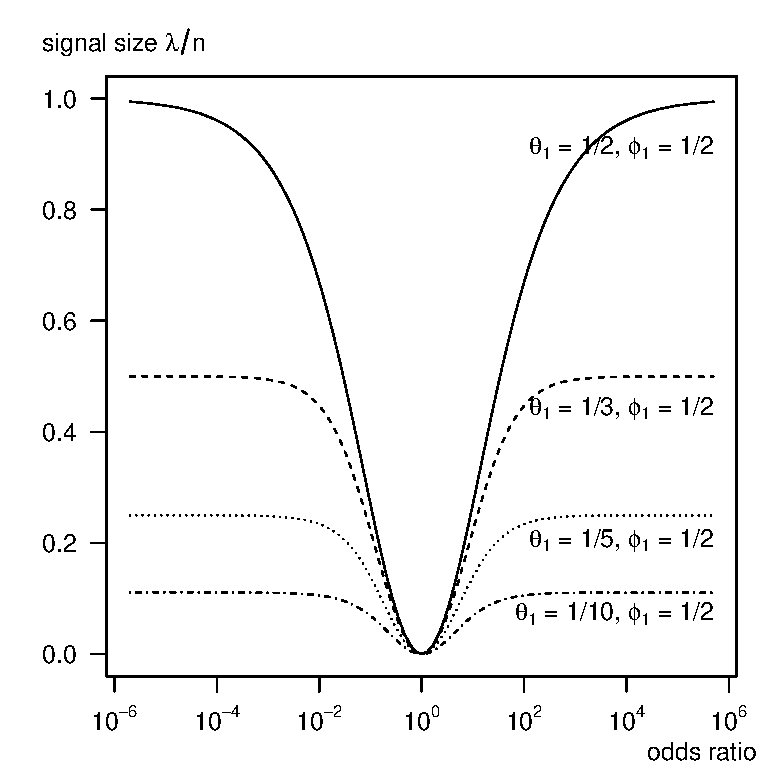
\includegraphics[width=0.49\textwidth]{./singal-vs-odds-p05}
      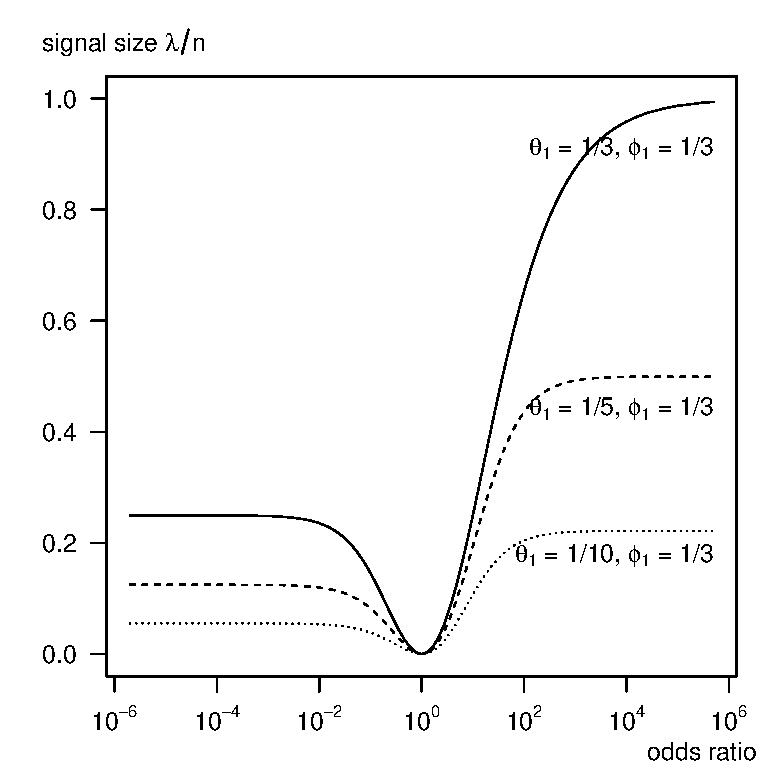
\includegraphics[width=0.49\textwidth]{./singal-vs-odds-p0333}            
      % 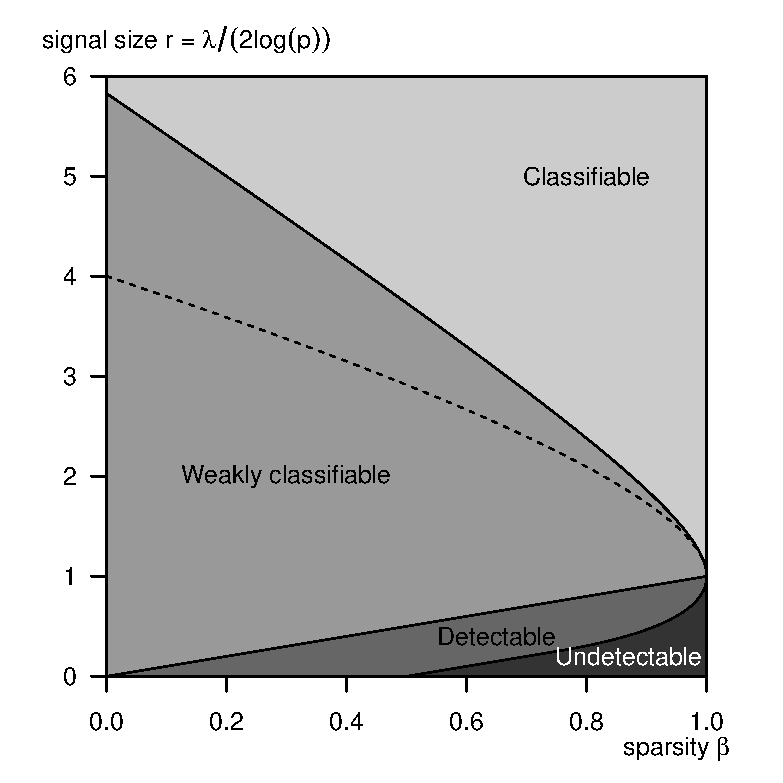
\includegraphics[width=0.35\textwidth]{./phase_diagram_chisquared.eps}
      \caption{Signal sizes per sample $w^2$ in chi-square tests as functions of odds ratios in 2-by-2 multinomial distributions, for selected marginal probabilities; see Relation \eqref{eq:signal-size-odds-ratio} in Proposition \ref{prop:signal-size-odds-ratio}.
      For fixed marginal distributions, extreme odds ratios imply stronger statistical signals at a given sample size.
      However, the signal sizes are bounded above by constants that depend on the marginal distributions; see Relations \eqref{eq:signal-size-upper-bound-1} and \eqref{eq:signal-size-upper-bound-2}.
      % Unbalanced marginal distributions -- or rare variants -- lead to smaller signal sizes at a given odds ratio.
      } 
      \label{fig:signal-vs-odds}
\end{figure}

\begin{corollary} \label{cor:signal-limits-OR}
The signal size as a function of the odds ratio $w^2(R)$ is decreasing on $(0,1)$ and increasing on $(1,\infty)$, with limits
\begin{equation} \label{eq:signal-size-upper-bound-1}
    \lim_{\text{R}\to0_+} w^2(\text{R}) = \min\left\{\frac{\phi_1\theta_1}{\phi_2\theta_2}, \frac{\phi_2\theta_2}{\phi_1\theta_1}\right\},
\end{equation}
and
\begin{equation} \label{eq:signal-size-upper-bound-2}
    \lim_{\text{R}\to+\infty} w^2(\text{R}) = \min\left\{\frac{\phi_1\theta_2}{\phi_2\theta_1}, \frac{\phi_2\theta_1}{\phi_1\theta_2}\right\}.
\end{equation}
\end{corollary}
Proof of Corollary \ref{cor:signal-limits-OR} is found in Appendix \ref{subsec:proof-signal-size-odds-ratio}. 

Corollary \ref{cor:signal-limits-OR} immediately implies that balanced designs with roughly equal number of cases and controls are not necessarily the most informative.

\begin{example}
In a study where a third of the recruited subjects carry the genetic variant positively correlated with the trait ($\theta_1=1/3$), an unbalanced design with $\phi_1=1/3$ would maximize $w^2$ at large odds ratios.
This unbalanced design is much more efficient compared to, say, a balanced design with $\phi_1=1/2$.
In the first case, the signal size can reach up to $w^2\approx1$, whereas  $w^2<1/2$ in the second.
This difference can also be read by comparing the dashed curve ($\theta_1=1/3,\phi_1=1/2$) in the left panel of Figure \ref{fig:signal-vs-odds}, with the solid curve ($\theta_1=1/3,\phi_1=1/3$) in the right panel of Figure \ref{fig:signal-vs-odds}.
\end{example}

\subsection{Optimal study designs and rare variants}
\label{subsec:optimal-design} 

For a study with a fixed budget, i.e., a fixed total number of subjects $n$, the researcher is free to choose the fraction of cases $\phi_1$ to be included in the study.
A natural question is how this budget should be allocated to maximize the statistical power of discovery, or equivalently, the signal sizes $\lambda=nw^2$.

In principal, Relation \eqref{eq:signal-size-odds-ratio} can be optimized with respect to the fraction of cases $\phi_1$ in order to find optimal designs, if the rest of the parameters are known and held constant.
In practice, this is not the case.
While $(\phi_1, \phi_2)$ can be controlled, the distributions of genotypes in the study are often unknown prior to data collection, and can change with the case-to-control ratio.

Fortunately, the conditional distributions of genotypes in the healthy control groups are often reported by existing studies, and are available in GWAS catalogs such as the NHGRI-EBI GWAS catalog \cite{macarthur2016new}.
% Assume (after appropriate relabelling, hence without loss of generality) that the first variant is associated with an increased risk of disease, and is henceforth referred to as the risk variant.
We denote the conditional frequency of the first genetic variant in the control group as $(f, 1-f)$, where
$$
f := \mu_{21} / \phi_2.
$$
The multinomial distribution is fully parametrized by the new trio: $(f, \phi_1, R)$.
\begin{center}
    \begin{tabular}{cccc}
    \hline
    & \multicolumn{2}{c}{Genotype} \\
    \cline{2-3}
    Probabilities & Variant 1 & Variant 2 & Total by phenotype \\
    \hline
    Cases & $\frac{\phi_1fR}{fR+1-f}$ & $\frac{\phi_1(1-f)}{fR+1-f}$ & $\phi_1$ \\
    Controls & $f(1-\phi_1)$ & $(1-f)(1-\phi_1)$ & $1-\phi_1$ \\
    \hline
    \end{tabular}
\end{center}
Proposition \ref{prop:signal-size-odds-ratio} may also be re-stated in terms of these parameters.

% Note that all these quantities refer to what is in the study, and differ from their counterparts in the general population.

\begin{corollary} \label{cor:signal-size-odds-ratio-conditional-frequency}
In the 2-by-2 multinomial distribution with marginals $(\phi_1, \phi_2 = 1-\phi_1)$, and conditional distribution of the variants in the control group $(f, 1-f)$,
Relation \eqref{eq:signal-size-odds-ratio} holds with $\theta_1 = {\phi_1fR}/{(fR+1-f)} + f(1-\phi_1)$ and $\theta_2 = 1-\theta_1$.
\end{corollary} 

The choice of $\phi_1$ now has a practical solution.

\begin{corollary} \label{cor:optimal-design}
In the context of Corollary \ref{cor:signal-size-odds-ratio-conditional-frequency},
the optimal design $(\phi^*_1, \phi^*_2)$ that maximizes the signal size per sample $w^2$ is prescribed by
\begin{equation} \label{eq:optimal-design}
    \phi_1^* = \frac{fR+1-f}{fR+1-f+\sqrt{R}}, \quad\text{and}\quad 
    \phi_2^* = 1-\phi_1^*,
\end{equation}
when the denominator in \eqref{eq:optimal-design} is non-zero; otherwise, $\phi_1^*=\phi_2^*=1/2$.
\end{corollary} 

Proof of Corollary \ref{cor:optimal-design} is found in Appendix \ref{subsec:proof-signal-size-odds-ratio}. 

Of particular interest in the genetics literature are genetic variants with very low risk alleles frequencies in the control group (i.e., $f\approx 0$), known as rare variants.
In such cases, Equation \eqref{eq:optimal-design} can be approximated by
\begin{equation} \label{eq:optimal-design-approx}
    \phi_1^* \approx \frac{1}{1 + \sqrt{R}}.
\end{equation}
To illustrate, for rare and adversarial factors ($f\approx0$ and $R>1$), the optimal $\phi_1^*$ is less than $1/2$.
Therefore, for studies under a fixed budget, controls should constitute the majority of the subjects in order to maximize power of discovering such variants.
On the other hand, for rare and protective factors ($f\approx0$ and $R<0$), the optimal $\phi_1^*$ is greater than $1/2$, and cases should be the majority.

\subsection{Power analysis in large-scale association screening studies}

% Specifically, we develop recipes to find suitable designs of association studies such that combination of the dimensionality $p$, sparsity $\beta$, and signal sizes $r$ of the problem lands in the desired region of risk control, as predicted by the results in Section \ref{sec:chisq-boundaries}.

% Of course, in applications, not all three of the parameters $(p, \beta, r)$ can be altered as we wish.
% In particular, the problem dimensions and sparsity levels are usually determined by the underlying physical processes.
% In the GWAS example, the number of genomic marker locations is determined by the chip used for gene sequencing, while the number of relevant genomic locations is a consequence of the biological process.
% Therefore, in order to achieve a desired level of error control, we can often only hope to influence the statistical signal sizes.


Returning to the problem of \emph{high-dimensional} marginal screenings for categorical covariates, we demonstrate with an example how results in Sections \ref{sec:chisq-boundaries} and \ref{sec:signal-size-odds-ratio} may be used for planning of prospective studies.

\begin{example}
In a GWAS with $p = 10^6$ genomic markers, researchers wish to locate genetic associations with the trait of interest\footnote{In practice, dependence among the genetic markers at different locations (known as linkage disequilibrium) decay as a function of their physical distances on the genome, the correlations of the resulting statistics are roughly independent except at short distances.}.
Specifically, the relevant genetic variants are expected to have risk allele frequencies of $0.01$, and odds ratios of at least $1.2$.
By Corollary \ref{cor:optimal-design}, the optimal design has a fraction of cases $\phi^* = 0.478$, yielding the statistical signal size per sample $w^2\approx9.00\times10^{-5}$ according to Corollary \ref{cor:signal-size-odds-ratio-conditional-frequency}.

If we wish to achieve exact-approximate support recovery in the sense of \eqref{eq:support-recovery-success}, Theorem \ref{thm:chi-squared-exact-approx-boundary} predicts that the signal size parameter $r$ has to be at least $\widetilde{g}(\beta)= 1$.
This signal size calls for a sample size of $n = \lambda / w^2 = 2r\log(p)/w^2 \approx 307,011$.
In a typically GWAS, a pair of alleles are sequenced for every marker location, bringing the required number of subjects in the study to $n/2 \approx 153,509$.
\end{example}


\begin{figure}
      \centering
      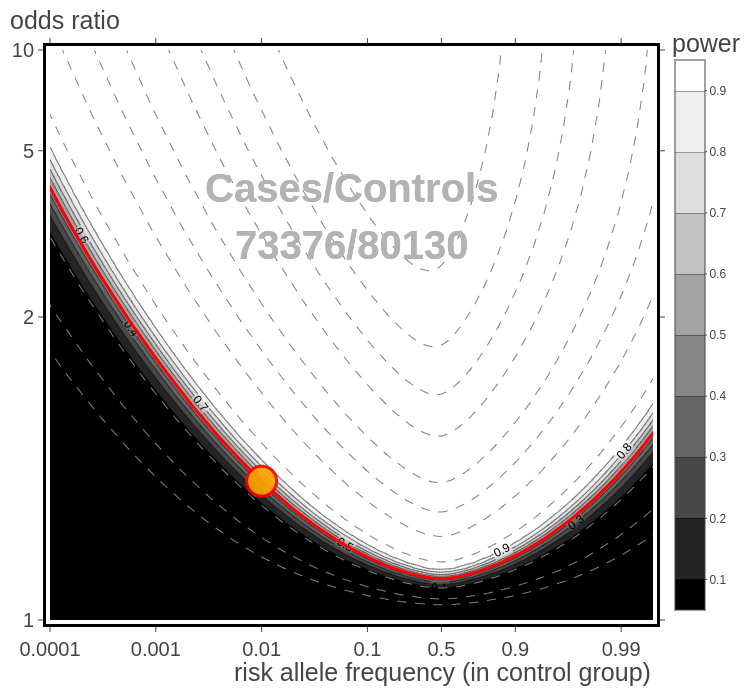
\includegraphics[width=0.49\textwidth]{./newplot.png} %OR-RAF_example.png}
      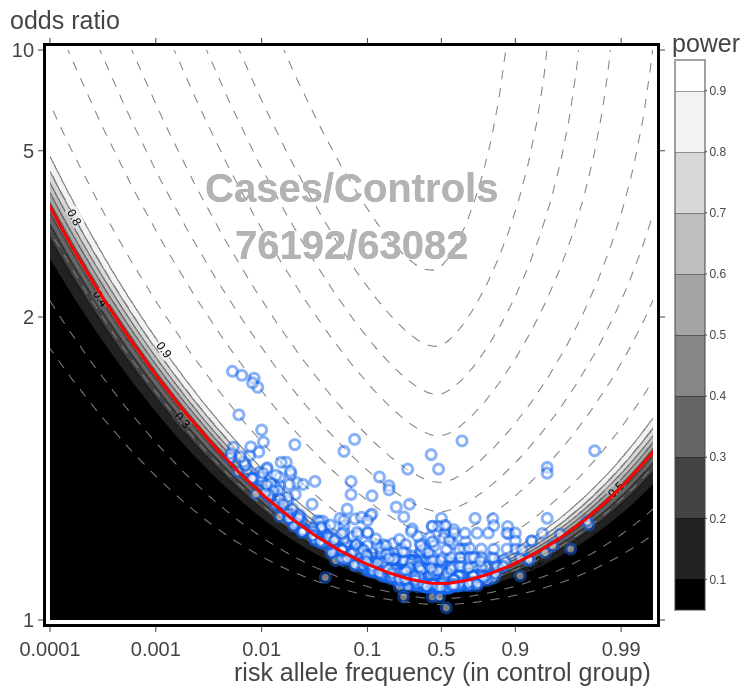
\includegraphics[width=0.49\textwidth]{./OR-RAF_BC_study.png}
      \caption{\fbox{Unfinished!!!} The OR-RAF diagram illustrating the sharp phase transition of marginal power in a GWAS study. 
      Blue circles: estimated odds ratios and risk allele frequencies of discovered associations in a recent GWA study \cite{michailidou2017association}.
      Red curve: the boundary of the phase transition for the exact-approximate support recovery problem $r=1$.
      Dashed curves: equi-power curves.} 
      \label{fig:OR-RAF_GWAS}
\end{figure}


In comparison, a more accurate power calculation, detailed in \cite{gao2019upass}, predicts that $n / 2 = 165,035$ subjects are needed, under the set of parameters ($p=10^6$, $f=0.01$, $R=1.2$) and $\mathrm{FWER}=0.05$, $\mathrm{FNR}=0.5$; this is $7\%$ higher than our crude asymptotic approximation.
% The accuracy of the asymptotic approximations, by nature of the statements in Theorem \ref{thm:chi-squared-exact-boundary} and \ref{thm:chi-squared-approx-boundary}, depends on how close the error metrics are to zero.
% For example, the number of subjects needed for $\mathrm{FWER}=\mathrm{FWNR}=0.01$ is $499,598$, an $8\%$ increase over the asymptotic prediction; at $\mathrm{FWER}=\mathrm{FWNR}=0.1$, this number becomes $398,996$, some $14\%$ lower than the asymptotic result.
In general, we recommend using the more precise approximations over the back-of-envelope asymptotics for planning prospective studies and performing systematic reviews;
a user-friendly web application implementing the precise approximations is provided in \cite{gao2019upass}.
Nevertheless, the insights gained from the asymptotic results cannot be supplanted.
